\documentclass[a4paper,10pt,twoside,openany]{book}

\usepackage[lang=hebrew]{maths}
\usepackage{hebrewdoc}
\usepackage{stylish}
\usepackage{lipsum}
\let\bs\blacksquare

\setlength{\parindent}{0pt}

%%%%%%%%%%%%
% Styling %
%%%%%%%%%%%%

\usepackage{enumitem}

%%%%%%%%%%%%%
% Counters  %
%%%%%%%%%%%%%

\setcounter{section}{1}     
            
%BIBLIOGRAPHY
\usepackage[
backend=biber,
style=alphabetic,
]{biblatex}
\addbibresource{bibliography.bib} %Imports bibliography file

\title{
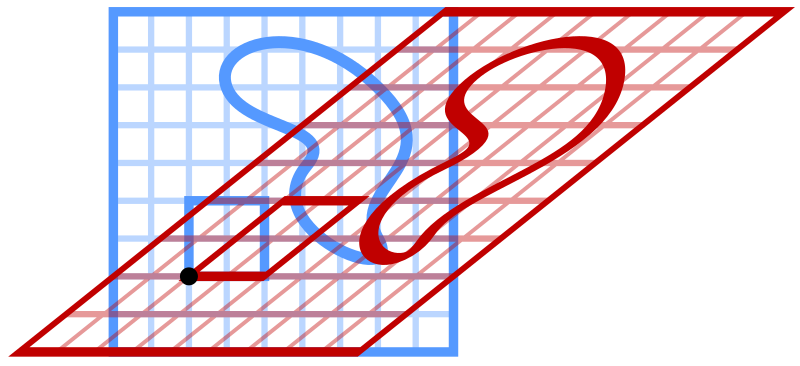
\includegraphics[width=6in]{images/front.png}\\
\vspace{30pt}
\Huge
אלגברה ב' (104168)
\\
אביב 2024
\\
רשימות תרגולים
\vspace{30pt}
\\
\huge
אלן סורני
\vspace{30pt}
\\
\Large
הרשימות עודכנו לאחרונה בתאריך ה־%
\today
}
\date{}

\begin{document}
\frontmatter
\maketitle
\tableofcontents

\mainmatter

\section*{סימונים}

\begin{itemize}
\item[-]
$\brs{n} = \set{1, \ldots, n}$.
\item[-]
$\sum_{i \in \brs{n}} a_i = \sum_{i=1}^n a_i = a_1 + a_2 + \ldots + a_n$
\item[-] $\Mat_{m \times n}\prs{\mbb{F}}$ הוא מרחב המטריצות עם
$m$
שורות ו־%
$n$
עמודות, עם מקדמים בשדה
$\mbb{F}$.
\item[-]
$\mbb{F}^n = \Mat_{n \times 1}\prs{\mbb{F}}$
\item[-]
$\Mat_{n}\prs{\mbb{F}} = \Mat_{n \times n}\prs{\mbb{F}}$
\item[-]
$\hom_{\mbb{F}}\prs{V,W}$
הוא מרחב ההעתקות הלינאריות
$V \to W$
כאשר
$V,W$
מרחבים וקטוריים מעל
$\mbb{F}$.
\item[-]
$\End_{\mbb{F}}\prs{V} = \hom_{\mbb{F}}\prs{V,V}$
\end{itemize}

\part{חלק ראשון - מרחבים שמורים}

\chapter{מטריצות מייצגות}

\section{הגדרות בסיסיות}

\begin{definition}[וקטור קואורדינטות]
יהי
$V$
מרחב וקטורי סוף־מימדי מעל שדה
$\mbb{F}$,
יהי
$B = \prs{v_1, \ldots, v_n}$
בסיס של
$V$
ויהי
$v \in V$.
\emph{וקטור הקואורדינטות של
$v$
לפי הבסיס
$B$}
הוא הוקטור
$\brs{v}_B = \pmat{\alpha_1 \\ \vdots \\ \alpha_n}$
כאשר
$\alpha_1, \ldots, \alpha_n \in \mbb{F}$
היחידים עבורם
\[\text{.}v = \sum_{i \in [n]} \alpha_i v_i \coloneqq \alpha_1 v_1 + \ldots + \alpha_n v_n\]
\end{definition}

\begin{remark}
ההעתקה
\begin{align*}
\rho_B \colon V &\to \mbb{F}^n \\
v &\mapsto \brs{v}_B
\end{align*}
היא איזומורפיזם לינארי.
\end{remark}

\begin{definition}[מטריצה מייצגת]
יהיו
$V,W$
מרחבים וקטורים סוף־מימדיים מעל אותו שדה
$\mbb{F}$
עם בסיסים
$B,C$
בהתאמה, ונסמן
\[\text{.} B = \prs{v_1, \ldots, v_n}\]
נסמן גם
$n \coloneqq \dim\prs{V}$
ו־%
$m \coloneqq \dim\prs{W}$.
עבור
$T \in \Hom_{\mbb{F}}\prs{V,W}$
נגדיר
\[\text{.} \brs{T}^B_C = \pmat{\vert & & \vert \\ \brs{T\prs{v_1}}_C & \cdots & \brs{T\prs{v_n}}_C \\ \vert & & \vert} \in \Mat_{m \times n}\prs{\mbb{F}}\]
\end{definition}

\begin{theorem}[כפל מטריצות]
תהי
$A \in \Mat_{m \times n}\prs{\mbb{F}}$
ויהי
$E = \prs{e_1, \ldots, e_m}$
הבסיס הסטנדרטי של
$\mbb{F}^n$.
אז:
\begin{enumerate}[label = (\roman*)]
\item
לכל
$i \in [m]$
מתקיים כי
$A e_i$
העמודה ה־%
$i$
של
$A$.
\item
לכל
$B = \pmat{\vert & & \vert \\ b_1 & \cdots & b_\ell \\ \vert & & \vert} \in \Mat_{n \times \ell}\prs{\mbb{F}}$
מתקיים
$AB = \pmat{\vert & & \vert \\ A b_1 & \cdots & A b_\ell \\ \vert & & \vert}$.
\end{enumerate}
\end{theorem}

\begin{exercisechap}
הראו שניתן לשחזר את ההגדרה של כפל מטריצות משתי התכונות במשפט.
\end{exercisechap}

\begin{remark}
ההעתקה
\begin{align*}
\eta^B_C \colon \Hom_{\mbb{F}}\prs{V,B} &\to \Mat_{m \times n}\prs{\mbb{F}} \\
T &\mapsto \brs{T}^B_C
\end{align*}
היא איזומורפיזם לינארי.
\end{remark}

\begin{proposition}
תהי
$T \in \Hom_{\mbb{F}}\prs{V,W}$
ויהיו
$B = \prs{v_1, \ldots, v_n}$
בסיס של
$V$
ו־%
$C$
בסיס של
$W$.
אז
\[\brs{T}^B_C \brs{v}_B = \brs{T\prs{v}}_C\]
לכל
$v \in V$.
\end{proposition}

\pagebreak
\begin{proof}
עבור
$v = v_i$
מתקיים
$\brs{T}^B_C \brs{v_i}_B = \brs{T}^B_C e_i$
וזאת העמודה ה־%
$i$
של
$\brs{T}^B_C$,
שהינה
$\brs{T\prs{v_i}}_C$
לפי ההגדרה.

אם
$v = \sum_{i \in [n]} \alpha_i v_i$
נקבל מלינאריות של
$T$
ושל
$\rho_B$
כי
\begin{align*}
\brs{T\prs{v}}_C &= \brs{T\prs{\sum_{i \in [n]} \alpha_i v_i}}_C
\\&= \brs{\sum_{i \in [n]} \alpha_i T\prs{v_i}}_C
\\&= \sum_{i \in [n]} \alpha_i \brs{T\prs{v_i}}_C
\\&= \sum_{i \in [n]} \alpha_i \brs{T}^B_C \brs{v_i}_B
\\&= \brs{T}^B_C \prs{\sum_{i \in [n]} \alpha_i \brs{v_i}_B}
\\&= \brs{T}^B_C \brs{\sum_{i \in [n]} \alpha_i v_i}_B
\\\text{,} \hphantom{\brs{T\prs{v}}_C} &= \brs{T}^B_C \brs{v}_B
\end{align*}
כנדרש.
\end{proof}

\begin{notation}
אם
$B$
בסיס של מרחב וקטורי סוף־מימדי
$V$
ואם
$T \in \End\prs{V}$,
נסמן
$\brs{T}_B \coloneqq \brs{T}^B_B$
ונקרא למטריצה זאת
\emph{המטריצה המייצגת של
$T$
לפי הבסיס
$B$}.
\end{notation}

\begin{notation}
יהי
$V$
מרחב וקטורי סוף־מימדי עם בסיסים
$B,C$.
נסמן
$M^B_C \coloneqq \brs{\id_V}^B_C$.
\end{notation}

\begin{notation}
אם
$A \in \Mat_{n\times n}\prs{\mbb{F}}$,
נסמן
\begin{align*}
T_A \colon \mbb{F}^n &\to \mbb{F}^n \\
\text{.} \hphantom{lalala} v &\mapsto Av
\end{align*}
\end{notation}

\begin{exercisechap}\label{ex:p(x+1)}
יהי
$V = \mbb{R}_3\brs{x}$
מרחב הפולינום הממשיים ממעלה לכל היותר
$3$,
תהי
\begin{align*}
T \colon \mbb{R}_3\brs{x} &\to \mbb{R}_3\brs{x} \\
p\prs{x} &\mapsto p\prs{x+1}
\end{align*}
ויהי
$B = \prs{1,x,x^2,x^3}$
בסיס של
$V$.
כיתבו את
$\brs{T}_B$.
\end{exercisechap}

\begin{solution}
לפי הגדרת המטריצה המייצגת,
עמודות
$\brs{T}_B$
הן
$\brs{T\prs{x^i}}_B$
עבור
$i \in \set{0,1,2,3}$.
מתקיים
\begin{align*}
T\prs{1} &= 1 \\
T\prs{x} &= x+1 = 1 + x \\
T\prs{x^2} &= \prs{x+1}^2 = 1 + 2x + x^2 \\
T\prs{x^3} &= \prs{x+1}^3 = 1 + 3x + 3x^2 + x^3
\end{align*}
ולכן
\begin{align*}
\brs{T\prs{1}}_B &= e_1 \\
\brs{T\prs{x}}_B &= e_1 + e_2 \\
\brs{T\prs{x^2}}_B &= e_1 + 2 e_2 + e_3 \\
\brs{T\prs{x^3}}_B &= e_1 + 3 e_2 + 3 e_3 + e_4
\end{align*}
ואז
\begin{align*}
\text{.} \brs{T}_B &= \pmat{1 & 1 & 1 & 1 \\ 0 & 1 & 2 & 3 \\ 0 & 0 & 1 & 3 \\ 0 & 0 & 0 & 1}
\end{align*}
\end{solution}

\begin{exercisechap}
יהי
$V = \Mat_{2 \times 2}\prs{\mbb{C}}$,
תהי
\begin{align*}
T \colon V &\to V \\
A &\mapsto \frac{1}{2} \prs{A - A^t}
\end{align*}
ויהי
\[E = \prs{E_{1,1}, E_{1,2}, E_{2,1}, E_{2,2}} \coloneqq \pmat{\pmat{1 & 0 \\ 0 & 0}, \pmat{0 & 1 \\ 0 & 0}, \pmat{0 & 0 \\ 1 & 0}, \pmat{0 & 0 \\ 0 & 1}}\]
\emph{הבסיס הסטנדרטי של
$V$}.
כיתבו את
$\brs{T}_E$.
\end{exercisechap}

\begin{proof}
כמו מקודם, נחשב את
$\brs{T\prs{E_{i,j}}}_E$
כיוון שאלו עמודות
$\brs{T}_E$.
מתקיים
\begin{align*}
T\prs{E_{1,1}} &= \frac{1}{2} \prs{E_{1,1} - E_{1,1}} = 0 \\
T\prs{E_{1,2}} &= \frac{1}{2} \prs{\pmat{0 & 1 \\ 0 & 0} - \pmat{0 & 0 \\ 1 & 0}} = \frac{1}{2} E_{1,2} - \frac{1}{2} E_{2,1} \\
T\prs{E_{2,1}} &= \frac{1}{2} \prs{E_{2,1} - E_{1,2}} = \frac{1}{2} E_{2,1} - \frac{1}{2} E_{1,2} \\
\text{,} T\prs{E_{2,2}} &= \frac{1}{2} \prs{E_{2,2} - E_{2,2}} = 0 \\
\end{align*}
לכן
\begin{align*}
\brs{T\prs{E_{1,1}}}_E &= 0 \\
\brs{T\prs{E_{1,2}}}_E &= \frac{1}{2} e_2 - \frac{1}{2} e_3 \\
\brs{T\prs{E_{2,1}}}_E &= -\frac{1}{2} e_2 + \frac{1}{2} e_3 \\
\brs{T\prs{E_{2,2}}}_E &= 0
\end{align*}
ואז
\begin{align*}
\text{,} \brs{T}_E &= \pmat{0 & 0 & 0 & 0 \\ 0 & \frac{1}{2} & -\frac{1}{2} & 0 \\ 0 & -\frac{1}{2} & \frac{1}{2} & 0 \\ 0 & 0 & 0 & 0}
\end{align*}
כנדרש.
\end{proof}

\begin{exercisechap}
יהי
$V = \Hom_{\mbb{R}}\prs{\mbb{R}^2, \mbb{R}}$
עם הבסיס
$B = \prs{f_1, f_2}$
כאשר
\begin{align*}
f_1\prs{\pmat{x \\ y}} &= x \\
\text{,} f_2\prs{\pmat{x \\ y}} &= y
\end{align*}
ותהי
\begin{align*}
\text{.} A &= \pmat{1 & 2 \\ 3 & 4} \in \Mat_{2 \times 2}\prs{\mbb{R}}
\end{align*}
מיצאו
$T \in \End_{\mbb{R}}\prs{V}$
עבורו
$\brs{T}_B = A$.
\end{exercisechap}

\begin{solution}
עבור
$T \in \End_{\mbb{R}}\prs{V}$
מתקיים
\[\text{.} \brs{T}_B = \pmat{\vert & \vert \\ \brs{T\prs{f_1}}_B & \brs{T\prs{f_2}}_B \\ \vert & \vert}\]
לכן נדרוש
\begin{align*}
\brs{T\prs{f_1}}_B &= \pmat{1 \\ 2} \\
\text{.} \brs{T\prs{f_2}}_B &= \pmat{3 \\ 4}
\end{align*}
אז
\begin{align*}
T\prs{f_1} &= f_1 + 2 f_2 \\
\text{.} T\prs{f_2} &= 3 f_1 + 4 f_2
\end{align*}
לכן, אם
$f \in V$
איבר כללי, נכתוב
\[f\pmat{x\\y} = \alpha x + \beta y = \alpha f_1 \pmat{x \\ y} + \beta f_2\pmat{x \\ y}\]
ונקבל כי
\begin{align*}
\prs{T\prs{f}}\pmat{x\\y} &= \prs{T\prs{\alpha f_1 + \beta f_2}}\pmat{x\\y}
\\&= \alpha T\prs{f_1}\pmat{x\\y} + \beta T\prs{f_2} \pmat{x\\y}
\\&= \alpha \prs{f_1 + 2 f_2}\pmat{x\\y} + \beta \prs{3 f_1 + 4 f_2} \pmat{x\\y}
\\ \text{.} \hphantom{\prs{T\prs{f}}\pmat{x\\y}} &= \alpha \prs{x + 2 y} + \beta \prs{3 x + 4y}
\end{align*}
\end{solution}

\begin{proposition}
תהיינה
$A,B \in \Mat_{m \times n}\prs{\mbb{F}}$
ונניח כי לכל
$v \in \mbb{F}^n$
מתקיים
$Av = Bv$.
אז
$A = B$.
\end{proposition}

\begin{proof}
מהנתון, מתקיים
$\prs{A - B}v = 0$
לכל
$v \in \mbb{F}^n$.
בפרט העמודה ה־%
$i$
של
$A-B$,
שהינה
$\prs{A - B}e_i$,
שווה ל־%
$0$.
לכן
$A - B = 0$.
\end{proof}

\begin{proposition}
יהיו
$U,V,W$
מרחבים וקטוריים סוף־מימדיים מעל אותו שדה
$\mbb{F}$
עם בסיסים
$B,C,D$
בהתאמה,
ותהיינה
\begin{align*}
S \in \Hom_{\mbb{F}}\prs{U,V} \\
\text{.} T \in \Hom_{\mbb{F}}\prs{V,W}
\end{align*}
אז
\[\text{.} \brs{T \circ S}^B_D = \brs{T}^C_D \brs{S}^B_C\]
\end{proposition}

\begin{proof}
לכל
$u \in U$
מתקיים
\begin{align*}
\brs{T}^C_D \brs{S}^B_C \brs{u}_B &= \brs{T}^C_D \brs{S\prs{u}}_C
\\&= \brs{T \circ S \prs{u}}_D
\\&= \brs{T \circ S}^B_D \brs{u}_B
\end{align*}
לכן
\[\text{,} \brs{T}^C_D \brs{S}^B_C = \brs{T \circ S}^B_D\]
כנדרש.
\end{proof}

\begin{proposition} \label{proposition:change-of-basis-through-isomorphism}
יהיו
$V,W$
מרחבים וקטוריים סוף־מימדיים מעל שדה
$\mbb{F}$
ותהי
$T \in \Hom_{\mbb{F}}\prs{V,W}$
חד־חד ערכית.

יהיו
\begin{align*}
B &= \prs{v_1, \ldots, v_n} \\
C &= \prs{u_1, \ldots, u_n}
\end{align*}
בסיסים של
$V$
ויהיו
\begin{align*}
B' &= \prs{T\prs{v_1}, \ldots, T\prs{v_n}} \\
\text{.} C' &= \prs{T\prs{u_1}, \ldots, T\prs{u_n}}
\end{align*}
אז
$B',C'$
בסיסים של
$\im\prs{T} = \set{T\prs{v}}{v \in V}$
וגם
$M^B_C = M^{B'}_{C'}$.
\end{proposition}

\begin{solution}
כיוון ש־%
$T$
חד־חד ערכית ועל התמונה, צמצום הטווח נותן איזומורפיזם
$T \colon V \riso \im\prs{T}$.
איזומורפיזם שולח בסיס לבסיס, לכן
$B',C'$
בסיסים.

כעת, לכל
$i \in [n]$
נכתוב
\begin{align*}
v_i &= \sum_{j \in \brs{n}} \alpha_{i,j} u_i
\end{align*}
ואז
\begin{align*}
\text{.} M^B_C e_i = \brs{v_i}_C = \pmat{\alpha_{i,1} \\ \vdots \\ \alpha_{i,n}}
\end{align*}
כמו כן,
\begin{align*}
T\prs{v_i}
&=
T\prs{\sum_{i \in [n]} \alpha_{i,j} u_j}
\\&=
\sum_{i \in [n]} \alpha_{i,j} T\prs{u_j}
\end{align*}
ולכן גם
\[\text{.} M^{B'}_{C'} e_i = \brs{T\prs{v_i}}_{C'} = \pmat{\alpha_{i,1} \\ \vdots \\ \alpha_{i,n}}\]
קיבלנו כי כל עמודות המטריצות שוות, ולכן יש שוויון.
\end{solution}

\begin{exercisechap}
תהי
$A \in \Mat_{n \times n}\prs{\mbb{F}}$
הפיכה.
\begin{enumerate}
\item יהי
$E$
הבסיס הסטנדרטי של
$\mbb{F}^n$.
מיצאו בסיס
$B$
של
$\mbb{F}^n$
עבורו
$A = M^B_E$.

\item
מיצאו בסיס
$C$
של
$\mbb{F}^n$
עבורו
$A = M^E_C$.

\item
יהי
$B$
בסיס של
$\mbb{F}^n$.
מיצאו בסיס
$C$
של
$\mbb{F}^n$
עבורו
$A = M^B_C$.

\item
יהי
$V$
מרחב וקטורי ממימד
$n \in \mbb{N}_+$
מעל
$\mbb{F}$,
יהי
$T \in \End_{\mbb{F}}\prs{V}$
איזומורפיזם
ויהי
$B = \prs{v_1, \ldots, v_n}$
בסיס של
$V$.
מיצאו בסיס
$C$
של
$V$
עבורו
$\brs{T}^B_C = A$.
\end{enumerate}
\end{exercisechap}

\begin{solution}
\begin{enumerate}
\item
אם
$B = \prs{v_1, \ldots, v_n}$,
מתקיים מההגדרה כי
\[\text{.} M^B_E = \pmat{\vert & & \vert \\ \brs{v_1}_E & \cdots & \brs{v_n}_E \\ \vert & & \vert} = \pmat{\vert & & \vert \\ v_1 & \cdots & v_n \\ \vert & & \vert}\]
לכן ניקח את
$\prs{v_1, \ldots, v_n}$
להיות עמודות
$A$,
לפי הסדר.

\item
לכל
$v \in \mbb{F}^n$
מתקיים
\[M^C_E M^E_C v = M^C_E \brs{v}_C = \brs{v}_E = v\]
ולכן
$M^E_C = \prs{M^C_E}^{-1}$.
אם ניקח
$C = \prs{u_1, \ldots, u_n}$
כאשר
$u_i$
העמודה ה־%
$i$
של
$A^{-1}$
נקבל מהסעיף הקודם כי
$M^C_E = A^{-1}$
ולכן
$M^E_C = \prs{A^{-1}}^{-1} = A$.
כלומר ניקח,
$u_i = A^{-1} e_i$.

\item
מתקיים
$M^B_C = M^E_C M^B_E$
לכן נרצה שיתקיים
$M^E_C M^B_E = A$
או במילים אחרות
$M^E_C = A \prs{M^B_E}^{-1} = A M^E_B$.
מהסעיף הקודם, נרצה
$C = \prs{u_1, \ldots, u_n}$
כאשר
$u_i$
העמודה ה־%
$i$
של
$\prs{A M^E_B}^{-1} = M^B_E A^{-1}$,
כלומר
\[\text{.} u_i = M^B_E A^{-1} e_i\]

\item
עבור כל בסיס
$C'$
מתקיים
$\brs{T}^B_{C'} = M^B_{C'} \brs{T}^B_B$
לכן נרצה
$M^B_C \brs{T}^B_B = A$.
כיוון ש־%
$T$
איזומורפיזם, המטריצה
$\brs{T}^B_B$
הפיכה, ולכן נרצה
$M^B_C = A \prs{\brs{T}^B_B}^{-1}$.
כעת, אם
$C = \prs{v_1, \ldots, v_n}$
נקבל לפי
\ref{proposition:change-of-basis-through-isomorphism}
עבור האיזומורפיזם
$\rho_B$
כי
$M^B_C = M^E_{\hat{C}}$
כאשר
$\hat{C} = \prs{\brs{v_1}_B, \ldots, \brs{v_n}_B}$.
לכן נחפש
$\hat{C}$
עבורו
$M^E_{\hat{C}} = A \brs{T}_B^{-1}$.
לפי הסעיף השני, נרצה
$\hat{C} = \prs{u_1, \ldots, u_n}$
עבור
\[\text{.} u_i = \prs{A \brs{T}_B^{-1}}^{-1} e_i = \brs{T}_B A^{-1} e_i\]
לכן
\[\text{.} v_i = \rho_B^{-1} \prs{\brs{T}_B A^{-1} e_i}\]
\end{enumerate}
\end{solution}

\begin{exercisechap}
יהי
$V = \mbb{C}_3\brs{x}$,
תהי
\begin{align*}
T \colon V &\to V \\
\text{,} \hphantom{lalala} p\prs{x} &\mapsto p\prs{x+1}
\end{align*}
יהי
$E = \pmat{1,x,x^2,x^3}$,
\emph{הבסיס הסטנדרטי}
ותהי
$A = \pmat{0 & 1 & 0 & 0 \\ 1 & 0 & 0 & 0 \\ 0 & 0 & 0 & 1 \\ 0 & 0 & 1 & 0}$.
כיתבו מפורשות בסיס
$C$
של
$V$
עבורו
$A = \brs{T}^E_C$.
\end{exercisechap}

\begin{solution}
לפי התרגיל הקודם, נרצה קודם
$\hat{C} = \prs{u_1, \ldots, u_4}$
כאשר
$u_i = \brs{T}_E A^{-1} e_i$.
חישבנו ב־%
\ref{ex:p(x+1)}
כי
\[\brs{T}_E = \pmat{1 & 1 & 1 & 1 \\ 0 & 1 & 2 & 3 \\ 0 & 0 & 1 & 3 \\ 0 & 0 & 0 & 1}\]
וניתן לראות כי
$A^2 = I$
כלומר
$A^{-1} = A$.
נשים לב כי
\begin{align*}
A e_1 &= e_2 \\
A e_2 &= e_1 \\
A e_3 &= e_4 \\
A e_4 &= e_3
\end{align*}
ואז נקבל
\begin{align*}
u_1 &= \brs{T}_E A^{-1} e_1 = \brs{T}_E e_2 = \pmat{1 \\ 1 \\ 0 \\ 0} \\
u_2 &= \brs{T}_E A^{-1} e_2 = \brs{T}_E e_1 = \pmat{1 \\ 0 \\ 0 \\ 0} \\
u_3 &= \brs{T}_E A^{-1} e_3 = \brs{T}_E e_4 = \pmat{1 \\ 3 \\ 3 \\ 1} \\
\text{,} u_4 &= \brs{T}_E A^{-1} e_4 = \brs{T}_E e_3 = \pmat{1 \\ 2 \\ 1 \\ 0}
\end{align*}
כלומר
\[\text{,} \hat{C} = \prs{\pmat{1 \\ 1 \\ 0 \\ 0}, \pmat{1 \\ 0 \\ 0 \\ 0}, \pmat{1 \\ 3 \\ 3 \\ 1}, \pmat{1 \\ 2 \\ 1 \\ 0}}\]
ולבסוף
\[\text{.} C = \prs{v_1, v_2, v_3, v_4} \coloneqq \prs{1+x, 1, 1+3x+3x^2+x^3, 1+2x+x^2}\]

ליתר ביטחון, נבדוק שהמטריצה המייצגת היא אכן
$A$.
מתקיים
\begin{align*}
T\prs{1} &= 1 = v_2 \\
T\prs{x} &= x+1 = v_1 \\
T\prs{x^2} &= \prs{x+1}^2 = 1+2x+x^2 = v_4 \\
T\prs{x^3} &= \prs{x+1}^3 = 1+3x+3x^2+x^3 = v_3
\end{align*}
ולכן
\begin{align*}
\brs{T}^E_C &= \pmat{\vert & \vert & \vert & \vert \\ \brs{T\prs{1}}_C & \brs{T\prs{x}}_C & \brs{T\prs{x^2}}_C & \brs{T\prs{x^3}}_C \\ \vert & \vert & \vert & \vert}
\\&= \pmat{\vert & \vert & \vert & \vert \\ \brs{v_2}_C & \brs{v_1}_C & \brs{v_4}_C & \brs{v_3}_C \\ \vert & \vert & \vert & \vert}
\\&= \pmat{\vert & \vert & \vert & \vert \\ e_2 & e_1 & e_4 & e_3 \\ \vert & \vert & \vert & \vert}
\\&= A
\end{align*}
כנדרש.
\end{solution}

\section{גרעין ותמונה}

\begin{definition}[גרעין של העתקה לינארית]
יהיו
$V,W$
מרחבים וקטורים מעל אותו שדה ותהי
$T \in \Hom\prs{V,W}$.
\emph{הגרעין של
$T$}
הוא
\[\text{.} \ker\prs{T} \coloneqq \set{v \in V}{T\prs{v} = 0}\]
\end{definition}

\begin{definition}[תמונה של העתקה לינארית]
יהיו
$V,W$
מרחבים וקטורים מעל אותו שדה ותהי
$T \in \Hom\prs{V,W}$.
\emph{התמונה של
$T$}
היא
\[\text{.} \im\prs{T} \coloneqq \set{T\prs{v}}{v \in V}\]
\end{definition}

\begin{definition}[דרגה של אופרטור לינארי]
יהיו
$V,W$
מרחבים וקטורים מעל אותו שדה ותהי
$T \in \Hom\prs{V,W}$.
\emph{הדרגה של
$T$}
היא
\[\text{.} \rank\prs{T} \coloneqq \dim \prs{\im\prs{T}}\]
\end{definition}

\begin{remark}
אם
$V,W$
סוף־מימדיים עם בסיסים
$B,C$
בהתאמה, אז
\[\text{.} \rank\prs{T} = \rank\prs{\brs{T}^B_C}\]
\end{remark}

\begin{theorem}[משפט המימדים]
יהי
$V$
מרחב וקטורי סוף־מימדי ויהי
$T \in \End\prs{V}$.
אז
\[\text{.} \dim V = \dim \im\prs{T} + \dim \ker\prs{T}\]
\end{theorem}

\begin{exercisechap}
יהי
$V$
מרחב וקטורי סוף־מימדי ויהי
$v \in V$.
מיצאו בסיס
$B$
של
$V$
עבורו
$\brs{v}_B = \pmat{1 \\ \vdots \\ 1}$.
\end{exercisechap}

\begin{solution}
נשלים את
$\prs{v}$
לבסיס
$B_0 = \prs{v_1, \ldots, v_n}$
של
$V$
כאשר
$v_1 = v$.
תהי
\begin{align*}
\text{.} A \ceq \pmat{1 & & & & \\
1 & 1 & & 0 & \\
\vdots & & \ddots & & \\
1 & & & 1 & \\
1 & 0 & \cdots & 0 & 1} \in \Mat_n\prs{\mbb{F}}
\end{align*}
$A$
הפיכה, ולכן מתרגיל קודם קיים בסיס
$B = \prs{u_1, \ldots, u_n}$
של
$V$
עבורו
$M^{B_0}_B = A$.
נקבל
\begin{align*}
\brs{v}_B &= \brs{\id_V v}_B
\\&=
\brs{\id_V}^{B_0}_{B} \brs{v}_{B_0}
\\&= A \pmat{1 \\ 0 \\ \vdots \\ 0}
\\ \text{.} \hphantom{\brs{v}_B} &= \pmat{1 \\ \vdots \\ 1}
\end{align*}
מפורשות, ראינו כי ניתן לקחת
\[\text{.} u_i = \rho_{B_0}^{-1}\prs{\brs{\id}_B A^{-1} e_i} = \rho_{B_0}^{-1}\prs{A^{-1}e_i}\]
\end{solution}

\begin{exercisechap}
יהי
$V$
מרחב וקטורי סוף־מימדי מעל שדה
$\mbb{F}$,
ותהי
$T \in \End_{\mbb{F}}\prs{V}$.
הראו כי
$\rank T = 1$
אם ורק אם יש בסיסים
$B,C$
ל־%
$V$
כך שכל מקדמי
$\brs{T}^B_C$
הם
$1$.
\end{exercisechap}

\begin{solution}
נניח כי יש בסיסים
$B,C$
כמתואר. אז
$\rank T = \rank \brs{T}^B_C = 1$.

בכיוון השני, נניח כי
$\rank T = 1$.
כלומר,
$\dim \im T = 1$.
ממשפט המימדים מתקיים
$\dim V = \dim \ker T + \dim \im T$,
לכן
\[\text{.} \dim \ker T = \dim V - \dim \im T = \dim V - 1\]
יהי
$n \ceq \dim V$
ויהי
\[\tilde{B} \ceq \prs{u_1, \ldots, u_{n-1}}\]
בסיס של
$\ker T$.

יהי
$w$
וקטור פורש של
$\im T$
ויהי
$C$
בסיס של
$V$
כך שמתקיים
$\brs{w}_C = \pmat{1 \\ \vdots \\ 1}$,
שקיים לפי התרגיל הקודם.
יהי
$v \ceq T^{-1}\prs{w}$,
ואז
$\prs{v, u_1, \ldots, u_{n-1}}$
בלתי־תלויים לינארית, כי
$v \notin \ker T$.
לכן זה בסיס של
$V$.
אז גם
$B \ceq \prs{v, v + u_1, \ldots, v + u_{n-1}}$
בסיס של
$V$
כי
המטריצה
\[\pmat{\vert & & \vert \\ \brs{v}_{\tilde{B}} & \cdots & \brs{v + u_{n-1}}_{\tilde{B}} \\ \vert & & \vert} = \pmat{1 & 1 & \cdots & 1 & 1 \\ 0 & 1 & & 0 & 0 \\ \vdots & & \ddots & & \vdots \\& 0 & & 1 & 0 \\
0 & & \cdots & 0 & 1}\]
הפיכה.

נסמן
$C = \prs{w_1, \ldots, w_m}$.
מתקיים
\[T\prs{v} = w = w_1 + \ldots + w_m\]
ולכל
$i \in [n-1]$
מתקיים
\begin{align*}
T \prs{v + u_i} &= T\prs{v} + T\prs{u_i}
\\&= T\prs{v} + 0
\\&= T\prs{v}
\\&= w_1 + \ldots + w_m
\end{align*}
לכן
$
\brs{T}^B_C
$
מטריצה שכל מקדמיה הם
$1$.
\end{solution}

\begin{exercisechap}
תהי
\begin{align*}
T \colon \mbb{R}_3\brs{x} &\to \mbb{R}_3\brs{x} \\
\text{.} p\prs{x} &\mapsto p\prs{-1}
\end{align*}
מיצאו בסיסים
$B,C$
של
$\mbb{R}_3\brs{x}$
עבורם
\[\text{.} \brs{T}^B_C = A \coloneqq \pmat{1 & 1 & 1 & 1 \\ 1 & 1 & 1 & 1 \\ 1 & 1 & 1 & 1 \\ 1 & 1 & 1 & 1}\]
\end{exercisechap}

\begin{solution}
ניקח בסיס
$\tilde{B} = \prs{b_1, b_2, b_3} \coloneqq \prs{x + 1, x^2 - 1, x^3 + 1}$
של
$\ker\prs{T}$,
כאשר זהו בסיס כי זאת קבוצה בלתי־תלוייה לינארית מגודל מקסימלי (הגרעין לכל היותר $3$ מימדי כי
$T \neq 0$).
מתקיים
$w \coloneqq -1 = T\prs{x}$
ואז
$\im\prs{T} = \Span_{\mbb{R}}\prs{w}$.
נחשב בסיס
$C$
עבורו
$\brs{w}_C = \pmat{1 \\ 1 \\ 1 \\ 1}$.
נשלים את
$\prs{v}$
לבסיס
\[\text{.} C_0 = \prs{v_1,v_2,v_3,v_4} \coloneqq \prs{-1,x,x^2,x^3}\]
המטריצה
\[X = \pmat{1 & 0 & 0 & 0 \\ 1 & 1 & 0 & 0 \\ 1 & 0 & 1 & 0 \\ 1 & 0 & 0 & 1}\]
הפיכה ולכן קיים בסיס
$C = \prs{u_1, u_2, u_3, u_4}$
עבורו
$M^{C_0}_C = X$,
כשראינו שאז
$\brs{w}_C = \pmat{1\\1\\1\\1}$.
כפי שראינו, ניתן לחשב את
$C$
לפי
$u_i = \rho_{C_0}^{-1}\prs{X^{-1} e_i}$.
מתקיים
\[X^{-1} = \pmat{1 & 0 & 0 & 0 \\ -1 & 1 & 0 & 0 \\ -1 & 0 & 1 & 0 \\ -1 & 0 & 0 & 1}\]
ולכן
\begin{align*}
u_1 &= \rho_{C_0}^{-1} \prs{\pmat{1 \\ -1 \\ -1 \\ -1}} = -1 -x - x^2 - x^3 \\
u_2 &= \rho_{C_0}^{-1} \prs{\pmat{0\\1\\0\\0}} = x \\
u_3 &= \rho_{C_0}^{-1} \prs{\pmat{0\\0\\1\\0}} = x^2 \\
\text{.} u_4 &= \rho_{C_0}^{-1} \prs{\pmat{0\\0\\0\\1}} = x^3
\end{align*}
כלומר,
$C = \prs{-1-x-x^2-x^3, x, x^2, x^3}$.

ניקח
$v = x \in V$
כך שיתקיים
$T\prs{v} = -1 = w$
ואז
\[B = \prs{v, v+b_1, v+b_2, v+b_3} = \prs{x, 2x+1, x^2+x-1, x^3 + x + 1}\]
כמו בתרגיל הקודם.

אכן, מתקיים
\begin{align*}
T\prs{x} &= -1 \\
T\prs{2x+1} &= -2 + 1 = -1 \\
T\prs{x^2 + x - 1} &= \prs{-1}^2 -1 - 1 = 1 - 2 = -1 \\
T\prs{x^3 + x + 1} &= \prs{-1}^3 -1 +1 = -1
\end{align*}
וגם
$\brs{-1}_C = \pmat{1 \\ 1 \\ 1 \\ 1}$,
לכן
\[\text{,} \brs{T}^B_C = \pmat{1 & 1 & 1 & 1 \\ 1 & 1 & 1 & 1 \\ 1 & 1 & 1 & 1 \\ 1 & 1 & 1 & 1}\]
כפי שרצינו.
\end{solution}

\printbibliography
\end{document}
